% \iffalse
\let\negmedspace\undefined
\let\negthickspace\undefined
\documentclass[journal,12pt,twocolumn]{IEEEtran}
\usepackage{cite}
\usepackage{amsmath,amssymb,amsfonts,amsthm}
\usepackage{algorithmic}
\usepackage{graphicx}
\usepackage{textcomp}
\usepackage{xcolor}
\usepackage{txfonts}
\usepackage{listings}
\usepackage{enumitem}
\usepackage{mathtools}
\usepackage{gensymb}
\usepackage{comment}
\usepackage[breaklinks=true]{hyperref}
\usepackage{tkz-euclide} 
\usepackage{listings}
\usepackage{gvv}                                        
\def\inputGnumericTable{}                                 
\usepackage[latin1]{inputenc}                                
\usepackage{color}                                            
\usepackage{array}                                            
\usepackage{longtable}                                       
\usepackage{calc}                                             
\usepackage{multirow}                                         
\usepackage{hhline}                                           
\usepackage{ifthen}                                           
\usepackage{lscape}
\newtheorem{theorem}{Theorem}[section]
\newtheorem{problem}{Problem}
\newtheorem{proposition}{Proposition}[section]
\newtheorem{lemma}{Lemma}[section]
\newtheorem{corollary}[theorem]{Corollary}
\newtheorem{example}{Example}[section]
\newtheorem{definition}[problem]{Definition}
\newcommand{\BEQA}{\begin{eqnarray}}
\newcommand{\EEQA}{\end{eqnarray}}
\newcommand{\define}{\stackrel{\triangle}{=}}
\theoremstyle{remark}

\newtheorem{rem}{Remark}
\begin{document}
\parindent 0px
\bibliographystyle{IEEEtran}
\title{Assignment 10.5.3\_13Q}
\author{EE23BTECH11219 - Rada Sai Sujan$^{}$% <-this % stops a space
}
\maketitle
\newpage
\bigskip
\section*{Question}
Find the sum of the first 15 multiples of 8. \\
\solution

    \begin{figure}[ht]
        \centering
        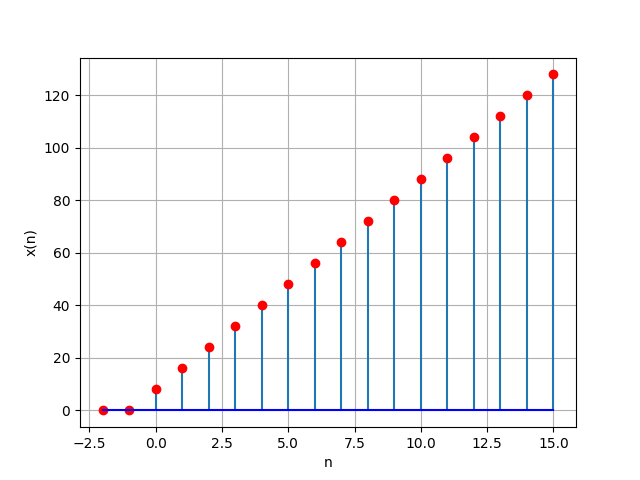
\includegraphics[width=\columnwidth]{figs/a.png}
        \caption{Plot of x(n) $vs$ n}
        \label{fig:10.5.3.13.1}
    \end{figure}
For an AP,
\begin{align}
    X\brak z &= \dfrac{ x\brak 0 }{1-z^{-1}} + \dfrac{dz^{-1}}{{(1-z^{-1})}^{2}}    \\
    \Rightarrow X\brak z &= \dfrac{8}{1-z^{-1}} + \dfrac{8z^{-1}}{{(1-z^{-1})}^{2}} \\
    &= \dfrac{8}{({1-z^{-1})}^{2}} , \;|z|>1    \\
    y\brak{n}&=x\brak{n}\ast u\brak{n}\\
    Y\brak{z}&=X\brak{z}U\brak{z}   \\
    \Rightarrow Y\brak{z}&=\brak{\dfrac{8}{({1-z^{-1})}^{2}}}\brak{\dfrac{1}{1-z^{-1}}}  \\
    &=\dfrac{8}{({1-z^{-1})}^{3}} , \;|z|>1
 \end{align}
 Using Contour Integration to find the inverse $Z$-transform,
\begin{align}
    \Rightarrow y(14)&=\dfrac{1}{2\pi j}\oint_{C}Y(z) \;z^{13} \;dz  \\
    &=\dfrac{1}{2\pi j}\oint_{C}\dfrac{8z^{13}}{({1-z^{-1})}^{3}} \;dz \\
    &=\sum\limits_{i}R_i
\end{align}
We can observe that there only a repeated pole at z=1,
\begin{align}
    \Rightarrow \sum\limits_{i}R_i &= R \\
    &=\dfrac{1}{\brak {2}!}\lim\limits_{z\to 1}\dfrac{d^{2}}{dz^{2}}\brak {{(z-1)}^{3}\dfrac{8z^{16}}{{(z-1)}^3}}   \\
    &=4\lim\limits_{z\to 1}\dfrac{d^2}{dz^2}(z^{16})   \\
    &=960
\end{align}
\begin{align}
    \therefore \boxed{y(14)=960}
\end{align}
\begin{table}[htbp]
    \def\arraystretch{1.5}
    \centering
    \begin{tabular}{|p{2.3cm}|p{2.3cm}|p{2.3cm}|}
    \hline
    PARAMETER & VALUE & DESCRIPTION \\ \hline
    x\brak0 & 8 & First term \\ \hline
    n & 15 & Number of terms \\ \hline
    d & 8 & common difference \\ \hline
    S &960 & Sum of n terms \\ \hline
    \end{tabular}
    \caption{Parameter Table1}
    \label{tab:1}
\end{table}

\end{document}
